\documentclass{standalone}
\usepackage{tikz}
\usetikzlibrary{arrows.meta, positioning, backgrounds, fit}
\usepackage{xcolor}
\colorlet{myred}{red!80!black}
\colorlet{myblue}{blue!80!black}
\colorlet{myblue}{myblue!80!black}
\colorlet{mygreen}{green!60!black}
\colorlet{myorange}{orange!70!red!60!black}
\colorlet{mydarkred}{red!30!black}
\colorlet{mydarkblue}{blue!40!black}
\colorlet{mydarkgreen}{green!30!black}
\begin{document}
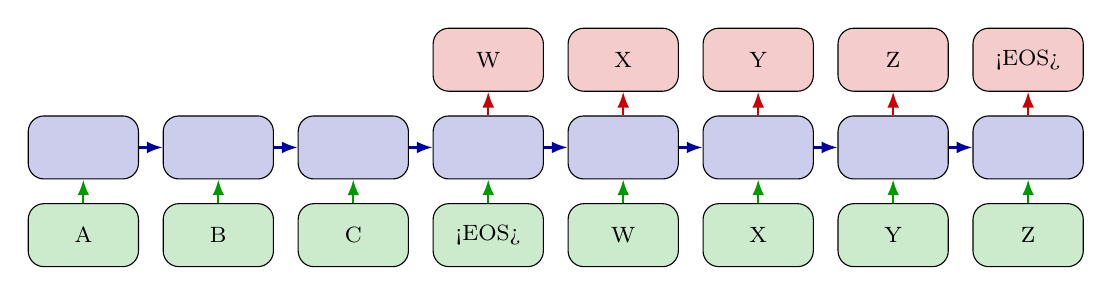
\begin{tikzpicture}[
    node distance=0.3cm and 0.3cm,
    every node/.style={minimum width=1.4cm, minimum height=0.8cm, align=center, draw=none, rounded corners=0.2cm},
    arrow/.style={-{Latex[length=2mm]}, thick}
]

% Many to Many (first version)
\begin{scope}[local bounding box=diagram3, xshift=8cm]
    \node[fill=white!20] (o31) {};
    \node[fill=white!20, right=of o31] (o32) {};
    \node[fill=white!20, right=of o32] (o33) {};
    \node[draw,fill=myred!20, right=of o33] (o34) {\footnotesize W};
    \node[draw,fill=myred!20, right=of o34] (o35) {\footnotesize X};
    \node[draw,fill=myred!20, right=of o35] (o36) {\footnotesize Y};
    \node[draw,fill=myred!20, right=of o36] (o37) {\footnotesize Z};
    \node[draw,fill=myred!20, right=of o37] (o38) {\footnotesize <EOS>};
    \node[draw,fill=myblue!20, below=of o31] (h31) {};
    \node[draw,fill=myblue!20, right=of h31] (h32) {};
    \node[draw,fill=myblue!20, right=of h32] (h33) {};
    \node[draw,fill=myblue!20, right=of h33] (h34) {};
    \node[draw,fill=myblue!20, right=of h34] (h35) {};
    \node[draw,fill=myblue!20, right=of h35] (h36) {};
    \node[draw,fill=myblue!20, right=of h36] (h37) {};
    \node[draw,fill=myblue!20, right=of h37] (h38) {};
    \node[draw,fill=mygreen!20, below=of h31] (i31) {\footnotesize A};
    \node[draw,fill=mygreen!20, below=of h32] (i32) {\footnotesize B};
    \node[draw,fill=mygreen!20, below=of h33] (i33) {\footnotesize C};
    \node[draw,fill=mygreen!20, below=of h34] (i34) {\footnotesize <EOS>};
    \node[draw,fill=mygreen!20, below=of h35] (i35) {\footnotesize W};
    \node[draw,fill=mygreen!20, below=of h36] (i36) {\footnotesize X};
    \node[draw,fill=mygreen!20, below=of h37] (i37) {\footnotesize Y};
    \node[draw,fill=mygreen!20, below=of h38] (i38) {\footnotesize Z};
    \foreach \i/\j in {h34/o34, h35/o35, h36/o36, h37/o37, h38/o38} {
        \draw[arrow, myred] (\i) -- (\j);
    }
    \foreach \i/\j in {i31/h31, i32/h32, i33/h33, i34/h34, i35/h35, i36/h36, i37/h37, i38/h38} {
        \draw[arrow, mygreen] (\i) -- (\j);
    }
    \foreach \i/\j in {h31/h32, h32/h33, h33/h34, h34/h35, h35/h36, h36/h37, h37/h38} {
        \draw[arrow, myblue] (\i) -- (\j);
    }
\end{scope}


\end{tikzpicture}
\end{document}